\section{Evaluation}\label{sec:eval}
\begin{figure*}[t]
	\centering 
        \scalebox{0.5}{
\includegraphics[width=\textwidth]{./fig/time/legend.pdf}}\\
    \centering
    \begin{subfigure}[t]{0.32\textwidth}
     \scalebox{1.0}{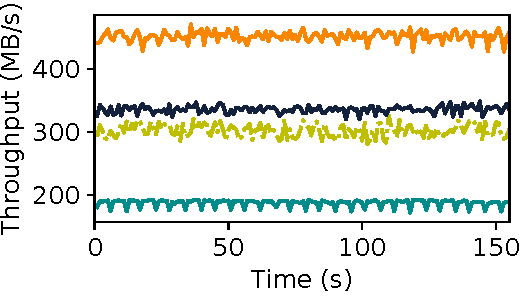
\includegraphics[width=\textwidth, page=1]{./fig/time/prealloc_bw.pdf}}
    %        \vspace{-1ex} 
        \caption{Single-Threaded 4KB Writes.}
        \label{fig:fio-4kb}
    \end{subfigure}
    \begin{subfigure}[t]{0.32\textwidth}
          \scalebox{1.0}{    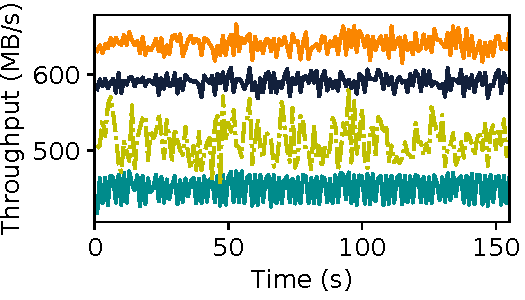
\includegraphics[width=\textwidth, page=1]{./fig/time/prealloc_16.pdf}}
          %     \vspace{-1ex}   
        \caption{Single-Threaded 16KB Writes.}
        \label{fig:fio-16kb}
    \end{subfigure}
    \begin{subfigure}[t]{0.32\textwidth}
           \scalebox{1.0}{   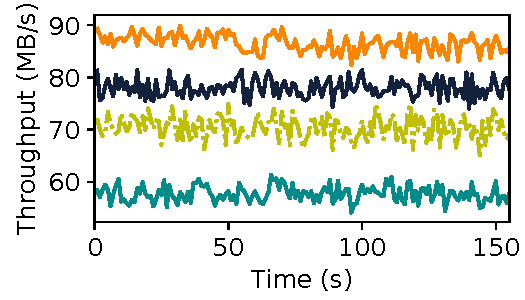
\includegraphics[width=\textwidth, page=1]{./fig/time/prealloc_bw_16thread.pdf}}
        %        \vspace{-1ex}   
        \caption{Multi-Threaded 4KB Writes.}
        \label{fig:fio:16th}
    \end{subfigure}
     %  \vspace{-2ex} 
    \caption{Real-time throughputs with Fio tests that simulate three different logging write patterns.}
    \label{Fig:fio}
    \vspace{-1ex}
\end{figure*}

%Let us
We evaluate \odes with real-world databases and prevalent benchmarks (Section~\ref{sec:eval:setup}).
%In particular, we
We particularly
aim to answer the following four questions.
\begin{itemize}[leftmargin=4mm]\setlength{\itemsep}{-\itemsep}
	\item Does \odes  indeed enable a fast shortcut path that outperforms
	conventional  path and SOTA design? (Section \ref{sec:eval:path})
	\item Does \odes manage to boost performance for a database with preallocated log files?	
	%utilizing its	shortcut path for logging writes? 
	(Section \ref{sec:eval:ob})
	\item Is \odes's strategy of reusing Ext4's {\em move-extent} feature efficient to
	%transfer blocks for resembling 
	resemble online preallocations? (Section \ref{sec:eval:preallocation})
	\item Does   enhanced  \odes improve performance for a database using
	a non-preallocated log file? (Section \ref{sec:eval:mysql})
\end{itemize}


\subsection{Experimental Setup}\label{sec:eval:setup}

{\bf Configurations.} We conduct  all experiments on an HP Z2 G4 workstation equipped with an Intel Core\textsuperscript{TM} i9-9900K CPU (16 cores) and 64GB DRAM. For storage, we set up  \odes on low-latency Samsung PM1725a with the PLP hardware support. 
The OS is Ubuntu 22.04.1 and the kernel version is 6.6.5.  %with Linux kernel 6.6.5.
 The  compiler is GCC/G++ 11.4.0.   

{\bf Testbeds.} % Without loss of generality, we 
We take %two databases, i.e., 
OceanBase (version 4.3.3) and  MySQL (version 8.4) %,
  to evaluate  \odes. The reason why they are used is threefold.
First, both of them are widely deployed.
Second, they are differently built on LSM-tree and B-tree, respectively. 
Third, % logging substantially affects their performances. Moreover, 
OceanBase mainly utilizes a preallocated log file, while MySQL has one preallocated log  (the redo log of InnoDB~\cite{mysql2013mysql})
and the other non-preallocated binlog, so with both databases we can % log (i.e., binlog \cite{mysql-binlog}).
%Hence, they enable us to
 comprehensively assess all aspects of \odes.
Additionally, we do not change their source codes, but edit a configuration file in them % one
to support
 \odes  identifying and intercepting logging writes.
%Both of them 

%{\bf Deployment.} 
%\odes generally demands no change to the source codes of databases.
%To deploy \odes for an application, we suggest that the  practitioners 
%could give a list of files that they intend to take \odes's path, while \odes will not deal with  other files. % will not be involved.
%For example, we employ \odes to cover logging writes for aforementioned two databases.
%In our evaluation, this is done by editing a configure file, which \odes digests and prepares
%for two databases. 

% For database evaluations, we configure OceanBase v4.3.3 with %parameter tuning based on
% recommended settings for local deployment \cite{githubObdeployexampleminilocalexampleyamlMaster}.
%OceanBase is an emerging database built on the LSM-tree concept \cite{DB:OceanBase:VLDB-2022}.

{\bf Baselines.} 
 We   evaluate \odes in two modes, i.e., \odes for fast mode (DAC) and \odes-S for strict permission checks (MAC).
Regarding the  concrete difficulty of reprogramming a complex database with SPDK or NVMeDirect (see \autoref{tab:mot:sota-comparison}),
we mainly  compare \odes to the stock storage  stack (denoted as `Vanilla') and  BypassD \cite{SSD:BypassD:ASPLOS-2024}.
The latter provides source codes with specialized IOMMU by emulation \cite{githubGitHubMultifacetBypassd}.
% The source codes of BypassD~\cite{githubGitHubMultifacetBypassd} have the emulation of its specialized IOMMU %hardware
%for per-file mappings.

%We evaluate \odes in two modes, i.e., \odes for fast mode (DAC) and \odes-S for strict permission checks (MAC).

%We intend to 
%, which respectively capture micro and macro performance metrics. 
%For SysBench, we execute the test on OceanBase, an emerging database built on the LSM-tree concept, thereby enabling 
%conduct a comprehensive assessment onto \odes with various tasks by using two benchmarks.
%We mainly use two benchmarks. 
{\bf Benchmarks.} 
We mainly use two benchmarks for evaluation.
The micro-benchmark is Fio. %~\cite{1fioFlex42:online}.
%by running two benchmarks, Fio and SysBench\cite{Sysbench38:online}.
The macro-benchmark is SysBench \cite{Sysbench38:online} that
  has multiple workloads reflecting production scenarios.
  %Some are write-dominant while  others continuously issue hybrid write and read transactions. % at the best effort.
We run SysBench on both databases.





% \begin{figure}[t]
%     \centering
%     
\includegraphics[width=0.45\textwidth, page=1, trim=20mm 42mm 0mm 0mm, clip]{./fig/oceanbase-sysbench-pm893/legend.pdf}
    
%     \begin{subfigure}[t]{0.48\textwidth}
%         \includegraphics[width=\textwidth, page=1]{./fig/oceanbase-sysbench-pm893/99p_all_insert.pdf}
%         \caption{99 percentile response time of all insert workload.}
%         \label{fig:o-sysbench-PM893-insert99p}
%     \end{subfigure}
%     \begin{subfigure}[t]{0.48\textwidth}
%         \includegraphics[width=\textwidth, page=1]{./fig/oceanbase-sysbench-pm893/99p_all_readwrite.pdf}
%         \caption{99 percentile response time of all read write workload.}
%         \label{fig:o-sysbench-PM893-readwrite99p}
%     \end{subfigure}
%     \caption{99 percentile response time for Oceanbase}
%     \label{Fig:99pResponseTime}
% \end{figure}

% \begin{figure}[t]
%     \centering
%     
\includegraphics[width=0.45\textwidth, page=1, trim=20mm 42mm 0mm 0mm, clip]{./fig/oceanbase-sysbench-pm893/legend.pdf}
    
%     \begin{subfigure}[t]{0.48\textwidth}
%         \includegraphics[width=\textwidth, page=1]{./fig/oceanbase-sysbench-pm893/tps_all_insert.pdf}
%         \caption{The throughput of all insert workloads.}
%         \label{fig:o-sysbench-PM893-insertTPS}
%     \end{subfigure}
%     \begin{subfigure}[t]{0.48\textwidth}
%         \includegraphics[width=\textwidth, page=1]{./fig/oceanbase-sysbench-pm893/tps_all_readwrite.pdf}
%         \caption{The throughput of all readwrite workloads.}
%         \label{fig:o-sysbench-PM893-readwriteTPS}
%     \end{subfigure}
% 	\caption{The throughput for sysbench workloads.}
%     \label{Fig:ThroughputWorkloads}
% \end{figure}

\subsection{Micro-benchmarking (Fio)}\label{sec:eval:path}
We simulate three typical patterns of database logging writes using Fio. %writing data to a file. % found in databases.
%We measure the throughput (MB/s) over time.
%TODO: where? which figure???? 
%%%In \autoref{Fig:fio}, the X axis represents time (seconds), and the Y axis denotes real-time throughput (MB/s).
% {\bf Single-Threaded 4KB Writes:}
%{\bf Logging I/O: flushing small records frequently:}
%We firstly simulate a common pattern of logging I/Os, i.e., frequently flushing small log records.
%We firstly simulate the behavior of databases such as OceanBase that flush small log records frequently.
Let us first study how \odes handles logging I/Os by which databases frequently flush  small log records.
 We configure a 1GB preallocated file. Each write is 4KB  followed by fdatasync. \autoref{fig:fio-4kb} shows that \odes exhibits the highest 
real-time throughput
  at the top,
  achieving  {2.4$\times$}  throughput
 compared to Vanilla.
 \odes hence manages to  exempt the software tax imposed on logging writes. Its  effectiveness % of \odes
 %This 
 is jointly achieved by all aspects of it. First,
leveraging the preallocation for a file results in a stable structural layout with deterministic block numbers.
 Second,
 using the in-memory Maco structure %for quick lookups
 %to
 % reorganize and buffer the per-file mappings %per file %maintained 
 %in the in-memory 
  minimizes the tedious cost of searching for a target block in the file's extent tree.
  % locating a target block by searching in the file's extent tree. % that will be tedious due to searching in .
 Third, the eBPF sitting between kernel and user spaces makes a bridge to pass
  each I/O request through the ioctl interfaces, which then allow delivering  data to the device with specific block numbers.
 They help to avoid the traversal of software layers including VFS, Ext4, bio layer, and I/O scheduler, thereby saving a lot of time.

% while \odes-S improves Fio by  {79\%}. 
In \autoref{fig:fio-4kb}, a comparison between the top curve and the middle fluctuating one tells that
\odes surpasses BypassD, by 49.2\% higher bandwidth on average for the entire writing task.
BypassD depends on a specialized  IOMMU for acceleration.
  %, originally intended to map memory addresses for I/O devices\cite{amd2007technology}. 
  Extending IOMMU to map in-file offsets to   block numbers risks interfering with IOMMU's main function.
   %which is neither documented in BypassD's literature \cite{SSD:BypassD:ASPLOS-2024} nor reflected in its emulated IOMMU code. 
  This may not only cause compatibility issues, but also degrade BypassD's performance and %, undermining 
  portability. In contrast, \odes is a fully all-in-software design. It is readily deployable on existing systems
  and also yields higher throughput than BypassD.
 %, which remains marginal compared to baseline gains.

% {\bf Single-Threaded 16KB Writes :}
%{\bf Simulate behavior of oltp write workload:}
In the second   test, we   engage a   thread in writing data to a 1GB preallocated file, but the I/O size per write  is  16KB. This is based on our measurement that
OLTP write transactions %of 
% Online Transaction Processing (OLTP) 
  empirically carry  16KB data on average. 
\autoref{fig:fio-16kb}  confirms that \odes outperforms Vanilla
by  {42.3\%} higher throughput.
Also, the real-time throughput of \odes is 24.8\% higher than that of BypassD on average, indicating that \odes is still more effective even
%than BypassD 
in case of larger   I/Os.

% {\bf Multi-Threaded 4KB Writes :}
%{\bf Simulate behavior of high concurrency logging}
\odes is optimized for scalability with per-core structures.
To assess its performance with multi-threads, we run 16 threads in parallel, each writing its own file, to match the number of CPU cores. As shown in \autoref{fig:fio:16th}, \odes produces  {47.4\%} higher throughput than Vanilla. 
As \odes builds parallel shortcut I/O paths for multi-threads and utilizes the distributed Maco structure, it manages to carry on concurrent write I/Os with low contention and  yield consistently high performance.


Lastly, let us compare \odes with \odes-S. % There is an average gap of 
The gaps are
 {25.8\%}, 7.7\%, and 34.1\%   between them with three test cases, reflecting 
 %The  {25.8\%} gap between \odes and \odes-S 
   the moderate cost of stricter permission checks for \odes-S.
That said,
%Given a log file,
this cost is avoidable in practice, because real-world databases are   unlikely to alter the write/read permissions of log files at runtime.
%while \odes-S achieves   {31.2\%} improvement. 

%For larger I/O and multi-threaded tests, \odes are 7.7\% and 34.1\% higher than \odes-S on average, respectively.
%These are because writing more data per file operation offsets the overhead of permission check  on each operation,
%while multiple faster  paths in parallel  amplify the impact of stricter checks.
%The narrower gap ({7.7\%})  between them 
%highlights the reduced overhead of permission checks  
%for larger I/Os. 
%with \odes-S improving by {34.1\%}

\begin{comment}
 

In summary, these
results justify \odes's potential 
in accelerating database logging writes.
% boosting write performance for database logging.
\odes bypasses almost all software layers, shortening the critical path and minimizing the runtime  tax.
% Stricter permission checks  in \odes-S impose   marginal overhead, proving that security enhancements need not compromise performance significantly. 
\end{comment}
%for database logging.


\subsection{Macro-benchmarking (OceanBase)}\label{sec:eval:ob}

\begin{figure*}[htbp]
    \centering
   \scalebox{0.9}{ 
\includegraphics[width=0.5\textwidth, page=1]{fig/eval/sysbench_ob/sysbench_ob_legend.pdf}}\\
    % --- Throughput ---
    \begin{subfigure}[t]{0.32\textwidth}
      \scalebox{0.9}{      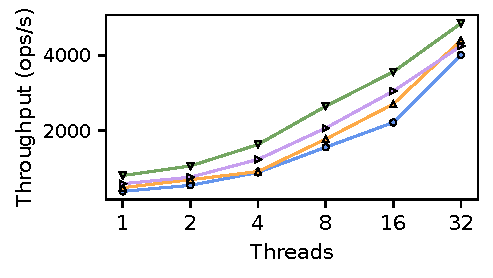
\includegraphics[width=\textwidth, page=1]{fig/eval/sysbench_ob/sysbench_ob_Write-Only_throughput2.pdf}}
      \vspace{-1ex}
        \caption{Throughput of Write-Only workload.}
        \label{fig:sysbench-ob-writeonly-tp}
    \end{subfigure}
    \begin{subfigure}[t]{0.32\textwidth}
           \scalebox{0.9}{       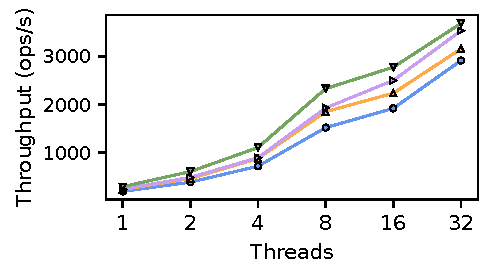
\includegraphics[width=\textwidth, page=1]{fig/eval/sysbench_ob/sysbench_ob_Read-Write_throughput2.pdf}}
                 \vspace{-1ex}
        \caption{Throughput of Read-Write workload.}
        \label{fig:sysbench-ob-readwrite-tp}
    \end{subfigure}
    \begin{subfigure}[t]{0.32\textwidth}
           \scalebox{0.9}{       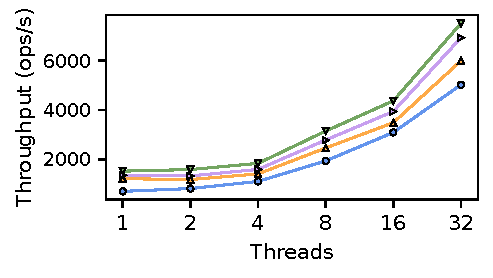
\includegraphics[width=\textwidth, page=1]{fig/eval/sysbench_ob/sysbench_ob_All Insert_throughput2.pdf}}
                 \vspace{-1ex}
        \caption{Throughput of All Insert workload.}
        \label{fig:sysbench-ob-insert-tp}
    \end{subfigure}
    % --- Latency ---
    \begin{subfigure}[t]{0.32\textwidth}
           \scalebox{0.9}{       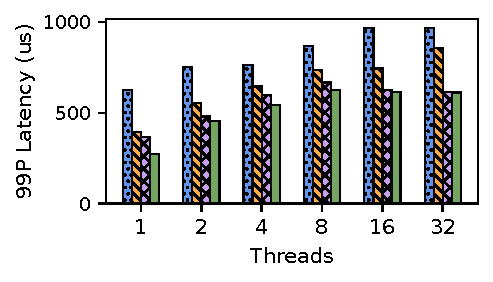
\includegraphics[width=\textwidth, page=1]{fig/eval/sysbench_ob/sysbench_ob_Write-Only_latency2.pdf}}
                 \vspace{-1ex}
        \caption{99P Latency of Write-Only workload.}
        \label{fig:sysbench-ob-writeonly-lat} 
    \end{subfigure}
    \begin{subfigure}[t]{0.32\textwidth}
            \scalebox{0.9}{      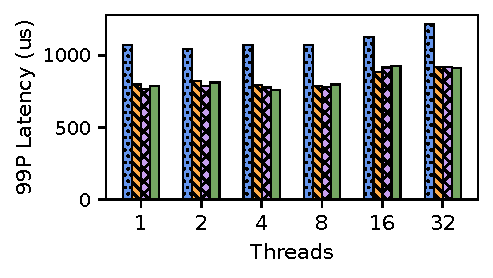
\includegraphics[width=\textwidth, page=1]{fig/eval/sysbench_ob/sysbench_ob_Read-Write_latency2.pdf}}
                  \vspace{-1ex}
        \caption{99P Latency of Read-Write workload.}
        \label{fig:sysbench-ob-readwrite-lat}
    \end{subfigure}
    \begin{subfigure}[t]{0.32\textwidth}
          \scalebox{0.9}{        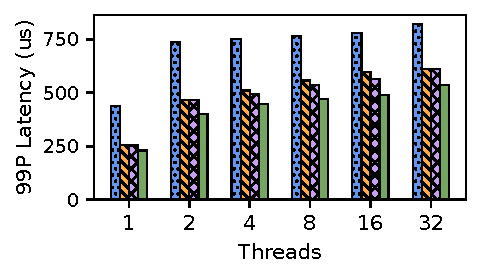
\includegraphics[width=\textwidth, page=1]{fig/eval/sysbench_ob/sysbench_ob_All Insert_latency2.pdf}}
                \vspace{-1ex}
        \caption{99P Latency of All Insert workload.}
        \label{fig:sysbench-ob-insert-lat}
    \end{subfigure}
%    \vspace{-2ex}
    \caption{Throughput and 99P tail latency of \odes on OceanBase with varying thread counts under SysBench workloads.}
    \label{fig:ob_sysbench}
        \vspace{-1ex}
\end{figure*}

Next
we employ \odes to substitute the path of OceanBase's logging writes.
We   run SysBench on OceanBase atop four configurations, i.e., the  Vanilla, BypassD, \odes-S, and \odes.
%SysBench includes multiple workloads. 
%Without loss of generality,
We take three representative OLTP workloads from SysBench for evaluation, i.e., OLTP-read\_write (mixed read/write transactions), OLTP-all\_insert (all insert transactions), and OLTP-write\_only (insert and update transactions). %Online Transaction Processing (OLTP) workloads are classic for DBs in production environments. OB developers used both workloads for testing\cite{oceanbaseSysbenchBenchmark}.
% \footnote{\scriptsize\url{https://en.oceanbase.com/docs/common-oceanbase-database-10000000001103501}}. 
% OceanBase supports concurrent transactions from multiple clients. 
 We vary the client threads as 1, 2, 4, 8, 16, and 32. %This will test \odes's performance and scalability. 
 For each client count, we use a 10-million-record table and execute each workload for 30 minutes. % (1,800 seconds). 
  \autoref{fig:ob_sysbench}  shows the throughput in operations per second (OPS) and 99P (the 99th percentile) tail latency. Regarding these results, we derive five observations. % from the above them. 

First, for write-intensive workloads with varying clients, \odes consistently surpasses Vanilla by offering higher throughput and lower tail latency. For the OLTP-write\_only workload with a single client, \odes achieves a throughput of  {2.1$\times$} compared to   
Vanilla, while the latter's 99P latency is up to {2.3$\times$} that of \odes. Similar performance trends are also observed with   other two workloads. 
\odes  minimizes the software overhead, as it
%OLTP-all\_insert shows similar performance.  
 skips over multiple software layers by routing logging I/Os through its own fast path.
Second, with 32 clients, the throughput and tail latency gaps reach 21.4\% and 62.3\%, respectively. 
\odes is  efficient and optimized for scalability.
% \odes bypasses most software layers, it has a much shorter critical path than the conventional stack. 
  OceanBase must handle contention among multiple threads, which leads to 
inevitable penalty in execution and offsets the effect of \odes. However, \odes is still performant.
%the time cost proportion in the storage stack decreases , \odes continues to outperform. 
Third, for OLTP-read\_write composed of mixed write and read transactions, \odes remains effective.  It  optimizes logging writes, 
while databases do not query a log file for read operations. In fact,
\odes places emphasis on logging writes and incurs no change to the original read path of OceanBase or other databases.  OceanBase's  user-space cache and the OS's page cache
help to retain high   hit rate and read throughput. 
Fourth, \odes outperforms BypassD by 31.1\% on average, which aligns with micro-benchmarking results. 
Finally, %comparing \odes and \odes-S reveals that 
OceanBase  never alters  access permissions or resizes log files. As shown in \autoref{fig:ob_sysbench}, stricter   checks for \odes-S still introduce  marginal overhead, e.g.,  18.5\% on OLTP-read\_write at 32 clients. 
Hence, users can consider either mode as needed, while \odes-S provides stronger protection at low cost.



\subsection{The Effect of Online Preallocation}\label{sec:eval:preallocation}

We have presented a test of on-the-fly space allocation in Section \ref{sec:motivation}  (see \autoref{fig:mot:prealloc-throughput}).
Before testing with a real-world   growing log file, we evaluate the effect of \odes's preallocation-like strategy that makes use of the {\em move-extent} feature of Ext4 as well as the io\_uring technique.
% , 
%in  Section \ref{sec:motivation}).
%which inspires us of
%the donor-based preallocation-like strategy. 
We repeat the same test onto \odes with a continuous  series of appending writes accumulated to overall 10GB, with 4KB, 8KB, 16KB, 32KB, 64KB, or 128KB
per write. We configure \odes to 
%call the {\em move-extent} feature and leverage io\_uring to 
asynchronously preallocate 64KB, 256KB, or 1MB from donor files.
\autoref{fig:eval:preallocation} shows the curves for three  preallocation sizes. We also include the results of conventional non-preallocation way
(the curve with dots). % for comparison.
Compared to it,
\odes increases  the throughput, for example, in terms of the typical 4KB I/O size,  by 3.3$\times$, 3.6$\times$, and 3.9$\times$ 
with three  increasing allocation spaces, respectively.
Section~\ref{sec:motivation} has tested another way to reserve space, i.e.,
calling fallocate on the critical path to reserve a batch of blocks prior to each
appending write (see \autoref{fig:mot:prealloc-throughput}), which serves as a
batched preallocation baseline. Calling fallocate in this way raises the throughput
of 4KB writes by 2.6$\times$, 3.2$\times$, and 3.4$\times$ over the conventional
non-preallocation way with the preallocation sizes of 64KB, 256KB, and 1MB, whereas
\odes reaches 3.3$\times$, 3.6$\times$, and 3.9$\times$ with the same three
preallocation sizes.
Both tests reserve the same amount of space and issue writes of the same size, so
the difference between the two groups of numbers does not come from performing
fewer allocations. The difference comes from moving the allocation off the critical
path and from the shortcut I/O path that \odes builds.
% (see Section \ref{sec:motivation}).
%These improves are all higher than the results discussed in
%Compared to the results shown in
% Section \ref{sec:motivation}.
These results justify that,
%\odes 
by employing donor files as a supplier of spaces and avoids on-demand allocations,
%on the critical path,
%thereby 
\odes
gains promising efficiency and  performance.
%using {\tt move-extent} and {\tt
	
	


\subsection{Macro-benchmarking (MySQL)}\label{sec:eval:mysql}

 


\begin{figure}[t]
    \centering
    \begin{minipage}[t]{0.24\textwidth}
        \centering
        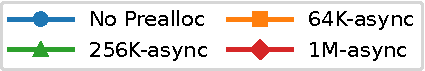
\includegraphics[width=0.94\textwidth, page=1]{./fig/eval/async-legend.pdf}
        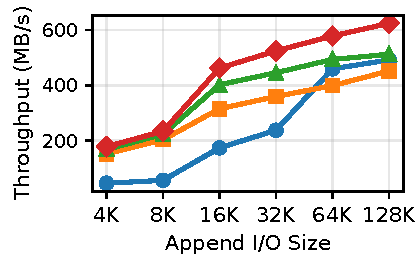
\includegraphics[width=\textwidth, page=1]{./fig/eval/backup-v/async-s.pdf}
   %  \vspace{-2ex}
        \caption{Impact of preallocation size.}
        \label{fig:eval:preallocation}
    \end{minipage}
    \label{fig:throughput_workloads}
    \begin{minipage}[t]{0.24\textwidth}
        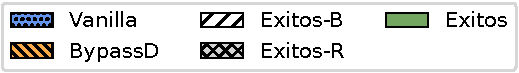
\includegraphics[width=\textwidth, page=1]{./fig/eval/backup-v/Mysql_legend_2.pdf}
        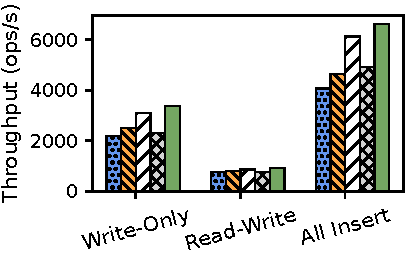
\includegraphics[width=\textwidth, page=1]{./fig/eval/backup-v/Mysql_BW_single.pdf}
   %          \vspace{-2ex}
        \caption{MySQL Throughput with SysBench workloads.}
        \label{fig:mysql_sysbench}
    \end{minipage}
  \vspace{-1ex}
\end{figure}

To comprehensively verify \odes's capability, we take MySQL for more tests. 
%MySQL is  a widely adopted   database.
 %, using the InnoDB as its storage engine~\cite{mysql2013mysql}. 
 We set up MySQL 8.4 with default  parameters.
%Unlike OceanBase's LSM-tree architecture, MySQL employs a traditional B+tree-based storage engine (InnoDB) with distinct logging characteristics: 
It has two main logs. One is the binlog that
%the binary log (binlog) 
uses appending writes for replication and recovery, while the InnoDB engine has a redo log that is preallocated and reused as a circular buffer~\cite{mysql2013mysql}. 
This dual-logging architecture exhibits an ideal scenario for evaluating \odes on 
both preallocated and growing log files.

Before testing with \odes, 
let us  figure out the impacts of two logs on the performance of MySQL.
We forcefully disable either log or both and
%, without loss of generality, execute
%By executing 
%the OLTP-write\_only workload 
execute OLTP workloads
of SysBench.
In the absence of both logs, the performance boosts by 109.0\% with the OLTP-write\_only workload. With 
either binlog or redo log disabled, the performance rises up by 60.8\% and 12.8\%, respectively.
Consequently, the aggregated cost of using both logs is significant, while the binlog brings  more performance overhead than the redo log.
%different log types.

We next %set up MySQL 8.0 with default  parameters and 
run three SysBench  workloads  as used in Section~\ref{sec:eval:ob}. 
Since there are two logs in MySQL, we make three variants, i.e., \odes handling writes to both logs, \odes-B handling binlog only, and \odes-R handling redo log only.
All of them apply the default DAC for permission checks. In particular,
\odes and \odes-B frequently call the {\em move-extent} and io\_uring
to extend the binlog file in a timely and asynchronous fashion,
resembling a preallocation effect on the fly.
%Similarly,
%we compare them to Vanilla and BypassD, and
Like what we have done with OceanBase,
 each test case runs for 30 minutes %with 1 concurrent client thread 
on a  table composed of 10 million records. 

%\autoref{fig:mysql_sysbench} presents the throughput comparison across five configurations: Vanilla, BypassD, \odes (both logs), \odes-B (binlog-only interception), and \odes-R (redo-only interception). Here, \odes applies our bypass optimization to both MySQL log types, \odes-B targets exclusively the append-only binlog, while \odes-R focuses solely on the preallocated InnoDB redo log.

\autoref{fig:mysql_sysbench} depicts the throughput comparison across five configurations.
With the OLTP-write\_only workload, \odes achieves 53.3\%  higher throughput than  Vanilla, demonstrating substantial performance gains by reshaping the path for both logs. \odes-B that optimizes only binlog writes, delivers 41.5\% improvement, while \odes-R shows modest 5.5\% gains by targeting the redo log only. 
This aligns with what we have obtained by disabling both logs or either one.
%This suggests that binlog operations contribute more significantly to the software tax in this workload. BypassD achieves 13.3\% improvement, substantially lower than all \odes variants.


For the OLTP-read\_write workload with mixed write and read transactions, \odes achieves 21.0\% higher throughput.
%workload shows more moderate but still meaningful improvements, with \odes achieving 21.0\% higher throughput. \odes-B improves performance by 15.2\% , while \odes-R shows minimal impact. 
 Read operations do not benefit from \odes's write-optimized shortcut path, and the workload's mixed nature reduces the relative impact of logging optimizations. 
 %The superior performance of \odes and \odes-B indicates that binlog writes are the primary bottleneck in mixed workloads.
As to  the OLTP-all\_insert workload, \odes yields the maximum potential, achieving 63.1\%
(i.e., 1.6$\times$) throughput improvement than Vanilla. This workload heavily stresses both  logs for MySQL, since each insert triggers file writes to binlog and redo log. 
Additionally, with all three workloads, %especially two write-intensive ones, 
\odes again outperforms BypassD,
 %BypassD achieves only 13.8\% improvement, 
 further confirming \odes's superiority. %  over hardware-dependent approach.



To summarize,
\odes reaps further efficiency and applicability with its preallocation-like strategy for non-preallocated log files.
%the donor-based preallocation-like strategy is an important part of \odes.
%Handling file writes for the growing binlog of MySQL confirms the efficacy of \odes.
Overall, the consistent performance gains with both OceanBase and MySQL 
justify that \odes's shortcut path effectively accelerates database logging writes.
%various writing patterns, including writes, overwrites, and appending writes
%with high flexibility. 
%We believe \odes is able to resolve writing bottlenecks in more applications.


 %trash
\begin{comment}
To sum up, these MySQL results reveal important insights: (1) binlog operations impose greater software tax than redo log operations under sysbench OLTP workloads (2) bypassing both log types yields the best performance, and (3) \odes's benefits extend across different database architectures and log types. The consistent performance improvements validate that our eBPF-based bypass approach effectively accelerates database logging operations, with flexibility to target specific bottlenecks based on workload characteristics.
\end{comment}